\section{Background}
\label{background}

In this section, we will introduce the basic ideas of the Bitcoin blockchain and particularly the main algorithm SHA-256, which we will implement. A basic understanding of these concepts is necessary to comprehend the underlying considerations of our architecture and optimizations. 

\subsection{Blockchain and Bitcoin}

The fundamental idea behind blockchain is the cryptographic linking of chunks of data, which are the blocks, in order to make the contained timestamp and data unalterable.
Therefore, every subsequent block contains not only the next part of the data but also a cryptographic hash digest of the previous block \cite{haberStornetta1991}.

This makes it difficult for attackers to modify the blocks afterwards, as altering a given block leads to a different hash digest\footnote{Although it is theoretically possible that we actually get the same hash digest again this is due to the currently unbroken collision resistance of SHA-256 very unlikely.}.
To keep the chain valid this new hash digest would have to be included in the next block, which would consequently alter that block as well. 
As a result, all of the blocks following the modified block have to be recalculated upon a change. 
If this recalculation is not possible in a fast way by the attacker, the regular chain will outpace the modified chain. 
The modified chain is then not recognized as real and ignored by the network, effectively mitigating the attack.

One of the first realizations of a blockchain was introduced by Satoshi Nakamoto in form of the cryptocurrency Bitcoin \cite{bitcoinPaper}. 
The currency uses a blockchain as a so called \emph{distributed ledger} to keep track of all transactions to avoid double spending and retroactive changes of the transaction history. 
As depicted in figure \ref{fig:bitcoinchain}, the linked part of the chain are the so-called block headers. 

\begin{figure}[h]
	\centering
	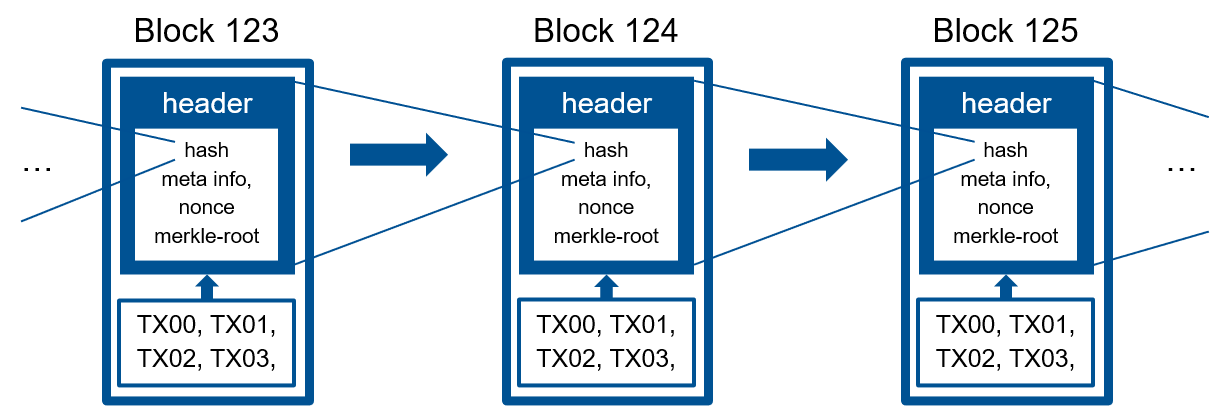
\includegraphics[width=\textwidth]{img/bitcoinchain.png}
	\caption[Schematic outline of the Bitcoin chain]{Schematic outline of the Bitcoin chain}
	\label{fig:bitcoinchain}
\end{figure}

The headers are linked through the cryptographic hash digest of the previous block header.
Furthermore, they include meta data describing the respective block as laid out in figure~ \ref{fig:headerformat}.
The transactions are integrated into the block's header via the \emph{merkle root}, which is a cryptographic hash digest summarizing them.

\begin{figure}[h]
	\centering
	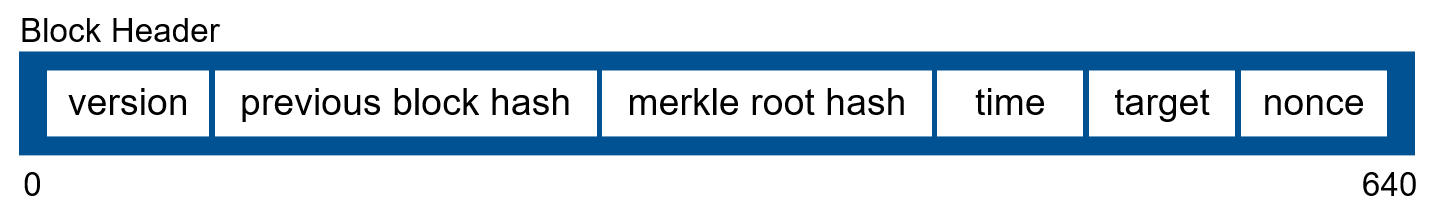
\includegraphics[width=\textwidth]{img/block-header-format.png}
	\caption[Bitcoin block header format]{Format of a Bitcoin block header}
	\label{fig:headerformat}
\end{figure}

In order to verify the blocks and transactions within them, the Bitcoin protocol uses a \emph{decentralized consensus system}. 
Every new block needs a so called \emph{Proof-of-Work} (PoW) in order to get accepted by the Bitcoin peer-to-peer network and finally to get appended to the chain.
In the case of Bitcoin, these proofs are the characteristic leading zero bits in the double-applied SHA-256 (SHA-256d) hash digest of the header, or, in more technical terms, a digest below a certain target value.
The action of searching for such a digest is called \emph{Bitcoin mining}.

Since the SHA-256 algorithm is designed in such a way that we cannot force to get certain properties in a hash digest, the only alternative is pure brute-force, which consumes a lot of calculation power. 
Therefore each PoW guarantees that, on average, a certain amount of computational power was put into the creation of a given block. 
If that amount is so high that even all network participants combined need several minutes per block, it is very hard for an individual attacker to be fast enough to rewrite the history of blocks as described earlier. 

The main part of the mining procedure is the search for the hash digest.
Because a hash function returns the same value for the same data every time, we have to change our header if the hash digest is not below the current target.
Such a change can be achieved by either modifying the merkle root, the timestamp or the nonce. The other fields (version, previous hash and target) are fixed for the current block.
Changing the merkle root is achieved by either including other transactions or changing a special field in the coinbase transaction, the first transaction which includes the incentive for finding a block. 
Both ways are quite costly since the merkle root has to be (partly) recalculated. 
Simpler ways of changing the header are direct increments of the dedicated 32-bit \emph{nonce} field or the timestamp in the header.
These options are the ones we will use later.

Finally to guarantee that the PoW still works even if a lot of miners join the Bitcoin network, the target value is regularly adjusted to keep the rate of blocks constant.
Therefore, we cannot hard-code the target value in this implementation and must require it to be read out from the header.

\subsection{SHA-256}
\label{sha256}

SHA-256 is the core algorithm of the Bitcoin proof-of-work and therefore the main algorithm we implement on our FPGA. It was officially introduced in the U.S. federal standard FIPS 180-2 in 2002 as part of the SHA-2 hash function family. 
It is a collision and preimage resistant hash function able to hash messages with a length of up to $2^{64}$ bit into 256-bit message digests \cite{FIPS180-2}. 

Preimage resistance means that it is infeasible to find a message for a given digest. 
This property makes the algorithm suitable for the verification of blocks in the Bitcoin protocol because the only way to find a valid block hash is through brute force, as already mentioned earlier.

Now we will have a look at the details of the hash digest calculation according to the FIPS standard \cite{FIPS180-2}. The algorithm can be split into two major parts, namely preprocessing and hash computation.

\subsubsection*{Preprocessing}

During preprocessing the message has to be prepared to fit the algorithm.
To make the subsequent subdivision into 512-bit chunks possible, the message is first padded to have a length in bits divisible by 512.
That is achieved by adding a $1$ bit to the end of the message $M$ and filling it with zeros until the length $l'$ of the result matches the equation $l' \equiv 448\mod 512$. Lastly, the length of the original message $M$ is appended as a 64-bit binary representation.

The subdivision into processable units is done by splitting the padded message $M'$ into $N$ 512 bit chunks ($M^{(1)},\dots,M^{(N)}$). 
Each of the chunks can also be seen as 16 32-bit words ($M_0^{(i)},\dots,M_{15}^{(i)}$).

Before starting the calculation it is also important to set the initial hash values $H_1^{(0)},\dots,H_7^{(0)}$ according to equation \eqref{eq:initHashvalues}.

\begin{equation}
\label{eq:initHashvalues}
	\begin{array}{l}
	H_{0}^{(0)}= \texttt{6a09e667} \\
	H_{1}^{(0)}= \texttt{bb67ae85} \\
	H_{2}^{(0)}= \texttt{3c6ef372} \\
	H_{3}^{(0)}= \texttt{a54ff53a} \\
	H_{4}^{(0)}= \texttt{510e527f} \\
	H_{5}^{(0)}= \texttt{9b05688c} \\
	H_{6}^{(0)}= \texttt{1f83d9ab} \\
	H_{7}^{(0)}= \texttt{5be0cd19} \\
	\end{array}	
\end{equation}

\subsubsection*{Hash computation}

The hash computation always processes one chunk at a time, so the following steps are executed for each of the $N$ blocks. 

\begin{enumerate}
	\item Extend the chunk $M^{(i)}$ to 64 message schedule words ($W_0,\dots, W_{63}$) according to equation \eqref{eq:extender}.
		
		\begin{equation}
		\label{eq:extender}
			W_{t}=
			\begin{cases}
				M_{t}^{(i)} & 0 \leq t \leq 15 \\
				\sigma_{1}\left(W_{t-2}\right)+W_{t-7}+\sigma_{0}\left(W_{t-15}\right)+W_{t-16} & 16 \leq t \leq 63
			\end{cases}
		\end{equation}
	
	\item Set the working variables $ a, \dots, h$ to the last hash values $H_1^{(i-1)},\dots,H_7^{(i-1)}$ respectively.
	
	\item In round $t$ from 0 to 63, process message schedule word $W_t$ according to equations \eqref{eq:computationValues} using functions \eqref{eq:shaFn1} and \eqref{eq:shaFn2} as well as constants $K_t$ \eqref{eq:shaConst}.
	
		\begin{equation}
		\label{eq:computationValues}			
			\begin{aligned}
				T_{1} &= h+\sum\nolimits_{1}(e)+C h(e, f, g)+K_{t}+W_{t} \\
				T_{2} &= \sum\nolimits_{0}(a)+M a j(a, b, c) \\
				h&=g \\	
				g&=f \\
				f&=e \\
				e&=d+T_{1} \\
				d&=c \\
				c&=b \\
				b&=a \\
				a&=T_{1}+T_{2}
			\end{aligned}
		\end{equation}

	\begin{equation}
	\label{eq:shaFn1}
	\begin{aligned}
		Ch(x, y, z) &= (x \wedge y) &&\oplus(x \wedge z) \\
		Maj(x, y, z) &= (x \wedge y) &&\oplus(x \wedge z) \oplus(y \wedge z)
	\end{aligned}
	\end{equation}
	
	\begin{equation}
	\label{eq:shaFn2}
	\begin{aligned}
		\sum\nolimits_{0}(x) &=\operatorname{ROTR}^{2}(x) &&\oplus \operatorname{ROTR}^{13}(x) &&\oplus \operatorname{ROTR}^{22}(x) \\
		\sum\nolimits_{1}(x) &= \operatorname{ROTR}^{6}(x) &&\oplus \operatorname{ROTR}^{11}(x) &&\oplus \operatorname{ROTR}^{25}(x) \\
		\sigma_{0}(x) &= \operatorname{ROTR}^{7}(x) &&\oplus \operatorname{ROTR}^{18}(x) &&\oplus \operatorname{SHR}^{3}(x) \\
		\sigma_{1}(x) &= \operatorname{ROTR}^{17}(x) &&\oplus \operatorname{ROTR}^{19}(x) &&\oplus \operatorname{SHR}^{10}(x)
    \end{aligned}
	\end{equation}
	
	Constants $K_t$ (from left to right) 

	\begin{equation}
	\label{eq:shaConst}
	\begin{aligned}
		\texttt{428a2f98} && \texttt{71374491} && \texttt{b5c0fbcf} && \texttt{e9b5dba5} && \texttt{3956c25b} && \texttt{59f111f1} \\
		\texttt{923f82a4} && \texttt{ab1c5ed5} && \texttt{d807aa98} && \texttt{12835b01} && \texttt{243185be} && \texttt{550c7dc3} \\
	    \texttt{72be5d74} && \texttt{80deb1fe} && \texttt{9bdc06a7} && \texttt{c19bf174} && \texttt{e49b69c1} && \texttt{efbe4786} \\
		\texttt{0fc19dc6} && \texttt{240ca1cc} && \texttt{2de92c6f} && \texttt{4a7484aa} && \texttt{5cb0a9dc} && \texttt{76f988da} \\
		\texttt{983e5152} && \texttt{a831c66d} && \texttt{b00327c8} && \texttt{bf597fc7} && \texttt{c6e00bf3} && \texttt{d5a79147} \\ 
		\texttt{06ca6351} && \texttt{14292967} && \texttt{27b70a85} && \texttt{2e1b2138} && \texttt{4d2c6dfc} && \texttt{53380d13} \\
		\texttt{650a7354} && \texttt{766a0abb} && \texttt{81c2c92e} && \texttt{92722c85} && \texttt{a2bfe8a1} && \texttt{a81a664b} \\
		\texttt{c24b8b70} && \texttt{c76c51a3} && \texttt{d192e819} && \texttt{d6990624} && \texttt{f40e3585} && \texttt{106aa070} \\
		\texttt{19a4c116} && \texttt{1e376c08} && \texttt{2748774c} && \texttt{34b0bcb5} && \texttt{391c0cb3} && \texttt{4ed8aa4a} \\
		\texttt{5b9cca4f} && \texttt{682e6ff3} && \texttt{748f82ee} && \texttt{78a5636f} && \texttt{84c87814} && \texttt{8cc70208} \\
						  && \texttt{90befffa} && \texttt{a4506ceb} && \texttt{bef9a3f7} &&\texttt{c67178f2}&&&&
	\end{aligned}
	\end{equation}

	\item After processing all words of a chunk the result is added to the old hash values:
		
		\begin{equation}
		\label{eq:computationAddition}	
			\begin{array}{l}
				H_{0}^{(i)}=a+H_{0}^{(i-1)} \\
				H_{1}^{(i)}=b+H_{1}^{(i-1)} \\
				H_{2}^{(i)}=c+H_{2}^{(i-1)} \\
				H_{3}^{(i)}=d+H_{3}^{(i-1)} \\
				H_{4}^{(i)}=e+H_{4}^{(i-1)} \\
				H_{5}^{(i)}=f+H_{5}^{(i-1)} \\
				H_{6}^{(i)}=g+H_{6}^{(i-1)} \\
				H_{7}^{(i)}=h+H_{7}^{(i-1)}
			\end{array}
		\end{equation}
		
\end{enumerate}

Lastly, after processing all $N$ chunks, the hash digest is the concatenation of the hash values:

\begin{equation}
	\text{message digest } = H_{0}^{(N)}\left\|H_{1}^{(N)}\right\| H_{2}^{(N)}\left\|H_{3}^{(N)}\right\| H_{4}^{(N)}\left\|H_{5}^{(N)}\right\| H_{6}^{(N)} \| H_{7}^{(N)}
\end{equation}

